% CREATED BY DAVID FRISK, 2018
\chapter{Behavior Studio}

Una vez definidas todas las herramientas que se van a utilizar para el desarrollo de este proyecto, se dedicará este capítulo para cubrir de forma extensa y precisa una de las patas fundamentales de este proyecto: la plataforma de \textit{machine learning} BehaviorStudio \footnote{https://jderobot.github.io/BehaviorStudio/}.
Para ello, se dará primero una visión general de la arquitectura de la aplicación, para acto seguido describir todos los detalles de la implementación llevada a cabo, así como los problemas que han surgido y las soluciones aportadas.

Este capítulo está dividido en 4 secciones principales que abordarán una pequeña introducción de la aplicación, el diseño de la arquitectura, los principales componentes que la componen y el modo de ejecución distribuido.

\section{Introducción}

BehaviorStudio es una plataforma de \textit{machine learning} de comportamientos basados en redes neuronales que permite conectar distintos \textit{software} inteligentes a un robot tanto real como simulado. La plataforma está ideada principalmente para la conducción autónoma a través del control visual utilizando como sensores principales las cámaras a bordo del robot, pero está preparada para el soporte de diferentes robots como: drones, robots industriales, domésticos, etc, y para diferentes sensores y actuadores. Esta plataforma está ideada para proporcionar una infraestructura accesible y flexible que permita ejecutar diferentes comportamientos complejos en coches autónomos implementados con diferentes técnicas como: \textit{deep learning} (redes de clasificación, regresión, recurrentes, LSTMs, ...), \textit{reinforcement learning} e incluso programación manual utilizando librerías de visión como OpenCV.

Esta plataforma está íntegramente desarrollada en Python dado que es uno de los lenguajes más utilizado por la comunidad en el desarrollo de aplicaciones de aprendizaje automático, al disponer de gran cantidad de librerías y herramientas creadas por la comunidad científica, tales como Numpy, Pytorch, OpenCV, etc.

Esta plataforma surge de la inspiración de otra plataforma similar en características denominada \textit{DetectionStudio} \footnote{https://jderobot.github.io/DetectionStudio/} desarrollada por miembros de la asociación JdeRobot \footnote{https://jderobot.github.io}.

\noindent BehaviorStudio proporciona la siguiente funcionalidad:

\begin{itemize}
    \item \textbf{Carga de cerebros}. Se pueden seleccionar diferentes modelos de comportamiento (modelos pre-entrenados) para su evaluación en la misma ejecución del programa.
    \item \textbf{Modificación "en caliente"}. BehaviorStudio permite la modificación del código del cerebro en ejecución sin necesidad de parar el programa, realizando carga dinámica de los algoritmos que gobiernan el robot.
    \item \textbf{Ejecución en diferentes plataformas}. La plataforma soporta entornos de ejecución locales (simulación en Gazebo) y remotos (robots reales).
    \item \textbf{Visualización}. Se incorpora la visualización de diferentes sensores como la cámara RGB o el láser.
    \item \textbf{Modo de ejecución distribuida}. Se permite ejecutar la lógica y la visualización en diferentes computadores (modo \textit{headless}), para permitir así que la capa de lógica corra empotrada en los robots, mientras que la capa de visualización se ejecute en un computador externo.
    \item \textbf{Creación de \textit{datasets}}. Se pueden grabar conjuntos de datos utilizando \textit{ROSBags} asociados a \textit{topics} de ROS.
\end{itemize}

La implementación de esta plataforma es flexible, lo que permite incorporar nueva funcionalidad como visualización de otros tipos de sensores de forma sencilla, o de nuevos marcos de trabajo como Tensorflow.

\section{Arquitectura}

El diseño de BehaviorStudio se puede ver en la Figura \ref{fig:architecture}. Como se puede observar, al tratarse de una aplicación que incorpora visualización, se ha implementado una arquitectura Modelo-Vista-Controlador (MVC). Se ha elegido esta arquitectura porque distingue muy bien la parte de lógica y la parte de visualización, disminuyendo el acoplamiento de componentes y facilitando la cohesión de los mismos. La parte inferior de esa infografía, bajo la etiqueta "\textit{Robotic Platform}", ilustra la capacidad que tiene BehaviorStudio de conectar con robots reales o simulados indistintamente, cambiando únicamente la configuración de la aplicación. Esto se consigue gracias a la estandarización en las comunicaciones que ofrece ROS en forma de \textit{topics}, para: tanto recibir la información sensorial de los sensores del robot, como para comandar órdenes a sus actuadores.

Los principales componentes de esta aplicación son los que se aprecian en la Figura \ref{fig:architecture}. Por simplicidad, este diagrama sólo muestra los componentes principales de BehaviorStudio, obviando el módulo de grabación de datasets que se explican en la sección \ref{sec:redata}. Se puede apreciar que los componentes de los sensores/actuadores, el piloto y el cerebro forman parte del Modelo en el MVC, y a su vez se observa el módulo controlador perteneciente a la capa controladora, y por último la interfaz de usuario (UI) que pertenece a la capa de vista del MVC. En la siguiente sección se explican detalladamente cada uno de los componentes \textit{software} implementados en esta aplicación.

\begin{figure}
  \centering
  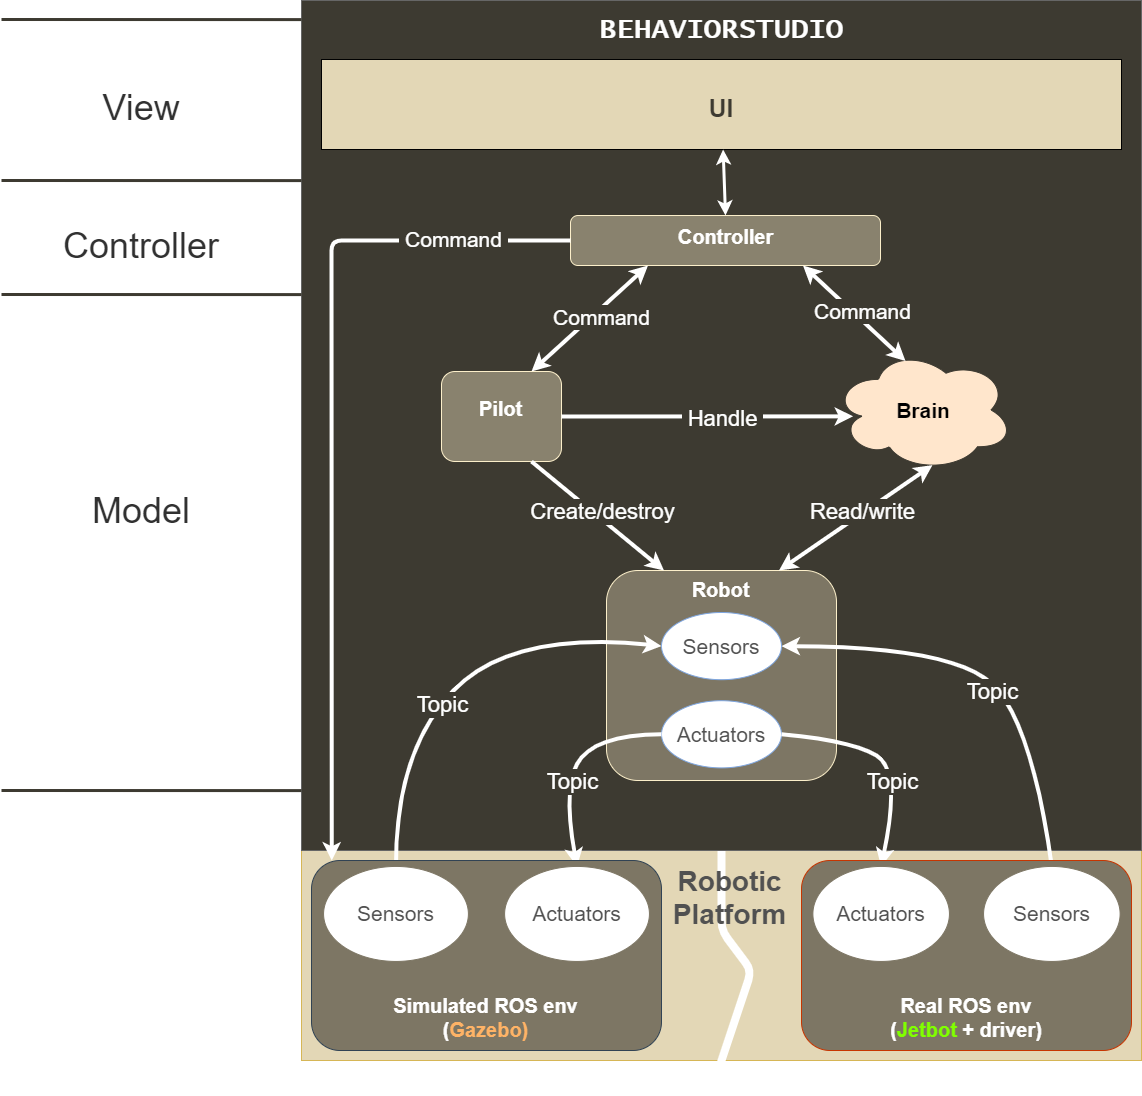
\includegraphics[width=.7\linewidth]{img/arquitectura}
  \caption{Arquitectura de BehaviorStudio}
  \label{fig:architecture}
\end{figure}

\section{Componentes}
\label{sec:components}

En esta sección se detallan los diferentes componentes que componen la arquitectura de la aplicación, tal como ilustra la figura \ref{fig:architecture}. Cada componente se explicará en una sección diferente para mayor claridad, para posteriormente abordar el modo de ejecución distribuida.

\subsection{Driver}
\label{sec:driver}

\textcolor{blue}{No sé si incluir esta sección. Es como el programa principal, que gestiona la ejecución, pero no sé si es interesante para el propósito de la memoria. Si es así la completo.}

El punto de entrada de la misma es el \textit{driver}. Este módulo gestiona la ejecución de toda la aplicación. Entre sus tareas se encuentra:

\begin{itemize}
    \item \textbf{Inicialización de componentes}. El \textit{driver} se encarga de crear todos los componentes necesarios para la ejecución del programa, entre ellos: el piloto,el interfaz de usuario, el simulador y el controlador.
    \item \textbf{Destrucción de componentes}. También se encarga de destruir todos los elementos creados cuando termina la ejecución.
\end{itemize}


\subsection{Piloto}
\label{sec:pilot}

El módulo principal de la aplicación es el piloto. Esta pieza se encarga principalmente de la creación tanto del robot (sensores y actuadores) como del cerebro que va a comandar al robot. El piloto tiene un hilo de ejecución que se actualiza periódicamente cada $ 60 ms $, donde en cada iteración se ejecuta una llamada al cerebro que esté cargado en ese momento, para que este tome una decisión en función del escenario en el que se encuentre en cada instante. En otras palabras, cada $ 60\ ms $ se realiza una llamada al método \lstinline{execute()} del cerebro cargado, que capturará información del sensor o sensores, realizará una inferencia sobre la información capturada y tomará una decisión sobre cómo debe actuar el robot en ese momento. Esto permite que el control sea reactivo, ya que se toman decisiones en cada instante en función de las percepciones del robot. Esto da pie a múltiples implementaciones de control visual tanto de lazo abierto (sin realimentación sobre el sistema) como de lazo cerrado (con realimentación sobre el sistema), todas reactivas.

\begin{figure}
  \centering
  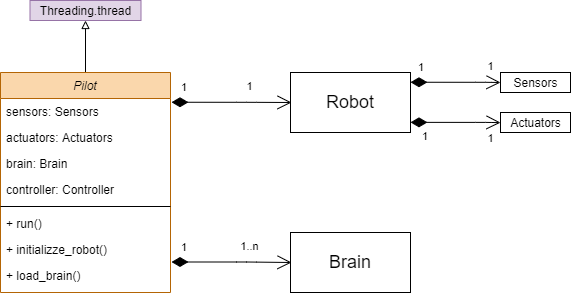
\includegraphics[width=.6\linewidth]{img/pilotuml}
  \caption{Diagrama de clases UML del componente pioto}
  \label{fig:pilotuml}
\end{figure}


Otra característica que se apuntó en la introducción es que BehaviorStudio permite el cambio de cerebros, además de cambios en el código fuente de forma dinámica sin necesidad de reiniciar la aplicación, esto es, en tiempo de ejecución. Es el piloto se encarga de realizar la carga y descarga de estos cerebros de forma dinámica que el usuario indique a través del interfaz de usuario.

En la Figura \ref{fig:pilotuml} se ilustra un diagrama de clases reducido de la clase piloto. Esta clase dispone de los métodos necesarios para crear un robot y cargar cerebros a placer de forma dinámica, además del hilo de ejecución principal.

\subsection{Robot - Sensores y actuadores}

Un elemento fundamental de los robots en general son sus sensores y actuadores, ya que sin ellos el robot sería incapaz de percibir (o sensar) ni de interactuar con el entorno. Por lo tanto, uno de los pilares principales de BehaviorStudio es la implementación del soporte de los sensores y actuadores del robot.

La implementación de este componente es sencilla, ya que se trata de un paquete de Python que incluye sendas clases \textit{Sensors} y \textit{Actuators}, que recibe una lista de sensores y actuadores con sus respectivos \textit{topics} desde el fichero de configuración de la aplicación. En la Figura \ref{fig:robouml} se puede ver un pequeño diagrama de clases UML que ilustra parcialmente la implementación de este componente. Esta implementación es flexible, ya que permite incluir una cantidad arbitraria de sensores y/o actuadores sin tener que modificar el código, sólamente modificando el fichero de configuración.

La forma en la que se construye un objeto sensor o actuador es especificando qué tipo de sensor se quiere construir, un identificador y el \textit{topic} de ROS asociado al publicador o subscriptor de ese sensor/actuador. Adicionalmente se podrá especificar configuración extra para cada sensor/actuador (requerirá la modificación del código). Todo esto se especifica a través de un fichero de configuración en formato YAML. En el Fragmento \ref{yml_rob} se puede ver un ejemplo de configuración para el robot F1.

\begin{tabular}{c}
\begin{lstlisting}[caption={Ejemplo de configuración en formato YAML},label=yml_rob]
Robot:
    Sensors:
        Cameras:
            Camera_0:
                Name: 'camera_0'
                Topic: '/F1ROS/cameraL/image_raw'
        Pose3D:
            Pose3D_0:
                Name: 'pose3d_0'
                Topic: '/F1ROS/odom'
    Actuators:
        Motors:
            Motors_0:
                Name: 'motors_0'
                Topic: '/F1ROS/cmd_vel'
                MaxV: 3
                MaxW: 0.3
    BrainPath: 'brains/f1/brain_f1_opencv.py'
    Type: 'f1'
\end{lstlisting}
\end{tabular}

Se pueden agregar tantos sensores o actuadores como tenga el robot en uso, pudiendo identificar cada uno de ellos con el identificador proporcionado en la etiqueta \textit{Name}. Los tipos de sensores soportados en la versión actual de BehaviorStudio son: cámaras RGB, láser, y pose3D. Por su parte, los actuadores soportados son: motores.

\begin{figure}
  \centering
  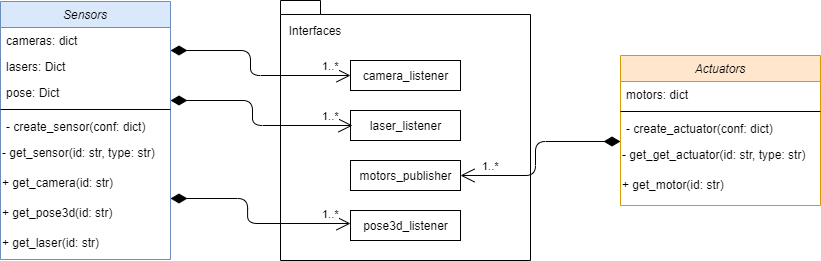
\includegraphics[width=1\linewidth]{img/robotuml}
  \caption{Diagrama de clases UML del componente Robot}
  \label{fig:robouml}
\end{figure}



\subsection{Cerebros neuronales}

El módulo de cerebros neuronales (llamado \textit{Brains}), es la pieza fundamental de BehaviorStudio, ya que es aquí donde residen los algoritmos que gobernarán a los robots. Como se aprecia en la Figura \ref{fig:architecture}, éste módulo conecta con los sensores y actuadores de los robots y es gestionado por el piloto, como se explicó en la sección \ref{sec:pilot}. Además tiene comunicación con el controlador, para que el usuario pueda interactuar con la carga de modelos, pausar o reanudar su ejecución, o modificar el código fuente todo en tiempo de ejecución. La conexión con los sensores y actuadores del robot, es fundamental para que el cerebro que esté en ejecución pueda realizar las inferencias a partir de los datos sensoriales, y comandar acciones al robot en función de las predicciones realizadas por las redes neuronales que gobiernan los robots.

Todos los módulos cerebro comparten un interfaz común, que "obliga" a seguir un estándar que democratiza todas las implementaciones que realicen los usuarios; así, un ejemplo de implementación de un cerebro sería como el que se muestra en el Fragmento \ref{brainex}. Como se puede observar, este cerebro es muy sencillo, el comportamiento que genera en el robot es que éste gira sobre su propio eje a $ 0.8\ rad/s $. 

Cada cerebro debe implementar una clase llamada \textit{Brain} instanciando en el constructor los sensores y actuadores del robot identificados por su nombre (en el caso del Fragmento \ref{brainex} \lstinline{camera_0} y \lstinline{motors_0} para la cámara y los motores respectivamente), además de una instancia del manejador de cerebros llamada \lstinline{handler}, que gestiona las comunicaciones con el módulo controlador. Dispone de un método \lstinline {update_frame()} que se encarga de actualizar la información que llega al interfaz de usuario con la visualización de los datos del sensor pertinente cada vez que se invoca. Por último, la función \lstinline {execute()}, es la encargada del bucle principal de ejecución que es llamada desde el módulo Piloto a un ritmo de ejecución determinado (ver sección \ref{sec:pilot}). 

En el caso de la Figura \ref{brainex}, cada vez que el método \lstinline{execute()} es invocado, se ejecutará lo siguiente: que el robot no avance (línea 13), que el robot gire sobre sí mismo a una velocidad de $0.8\ rad/s$ (línea 14), obtener una imagen de la cámara a bordo del robot (línea 15) y actualizar la información que se mostrará en la interfaz de usuario con la imagen capturada (línea 16). En la última instrucción, el primer argumento es \lstinline{frame_0}, que es el nombre del cuadro donde se mostrará la imagen capturada de la cámara del robot en el interfaz de usuario. Esto se explicará con más detalle en la sección \ref{sec:ui}.

\begin{tabular}{c}
\begin{lstlisting}[caption={Ejemplo de implementación de cerebro no neuronal},label=brainex,style=Python] 
class Brain:
    
    def __init__(self, sensors, actuators, handler=None):
       
        self.camera = sensors.get_camera('camera_0')
        self.motors = actuators.get_motor('motors_0')
        self.handler = handler

    def update_frame(self, frame_id, data):
        self.handler.update_frame(frame_id, data)

    def execute(self):
        self.motors.sendV(0)
        self.motors.sendW(0.8)
        image = self.camera.getImage().data
        self.update_frame('frame_0', image)
\end{lstlisting}
\end{tabular}


La estructura de este módulo se observa en la Figura \ref{fig:braindir}, donde se puede apreciar la estructura del árbol de ficheros que contienen el código del comportamiento. Como se puede ver, está dividido a nivel de robot con el objetivo de estructurar todos los cerebros a un mismo nivel de abstracción y que se sencillo para los usuarios saber dónde incluir sus algoritmos. Cada uno de los ficheros \lstinline{*.py} dentro de los directorios contiene un cerebro neuronal con comportamientos diferentes, así el fichero \lstinline{brain_f1_dummy.py} corresponde al código mostrado en el Fragmento \ref{brainex}. El fichero \lstinline{brain_handler.py} corresponde al manejador de cerebros, que es la clase que se encarga de gestionar la comunicación de cada cerebro con el controlador, que, como se explica en la sección \ref{sec:controller}, es el módulo encargado de comunicar la lógica de la aplicación con la capa de visualización.

Como se apuntó en la introducción de este capítulo, la plataforma está ideada para centrarse en la conducción autónoma con control basado en visión, pero esta figura ilustra muy bien que BehaviorStudio está preparada para soportar más tipos de robots y comportamientos.

\begin{figure}
\centering
\begin{forest}
  for tree={
    font=\ttfamily,
    grow'=0,
    child anchor=west,
    parent anchor=south,
    anchor=west,
    calign=first,
    inner xsep=7pt,
    edge path={
      \noexpand\path [draw, \forestoption{edge}]
      (!u.south west) +(7.5pt,0) |- (.child anchor) pic {folder} \forestoption{edge label};
    },
    % style for your file node 
    file/.style={edge path={\noexpand\path [draw, \forestoption{edge}]
      (!u.south west) +(7.5pt,0) |- (.child anchor) \forestoption{edge label};},
      inner xsep=2pt,font=\small\ttfamily
                 },
    before typesetting nodes={
      if n=1
        {insert before={[,phantom]}}
        {}
    },
    fit=band,
    before computing xy={l=15pt},
  }  
[brains
  [brain\_handler.py,file]
  [f1
    [brain\_f1\_dummy.py,file]
    [brain\_f1\_classification.py,file]
    [...,file]
  ]
  [car
    [brain\_car\_dummy.py,file]
    [...,file]
  ]
  [drone
    [...,file]
  ]
  [...,file]
]
\end{forest}
\caption{Estructura de directorios de cerebros neuronales}
\label{fig:braindir}
\end{figure}


\subsection{Controlador}
\label{sec:controller}


\subsection{Grabación de \textit{datasets}}
\label{sec:redata}


\subsection{Interfaz de usuario - GUI}
\label{sec:ui}

\subsubsection{Interfaz por terminal - TUI}
mencionar que la motivacion es que se pudiera manejar toda la aplicacion en el robot sin necesidad de capa de visualizacion externa.

¡¡¡AL ANEXO!!!!



\section{Modos de ejecución distribuido}
\label{sec:headless}

mencionar la necesidad de liberar de computo al robot y que no tiene sentido meter visualizacion en el mismo.